\documentclass{beamer}
\usepackage{clrscode}
\usepackage{graphicx}
\usepackage{booktabs}
\usepackage[most]{tcolorbox}
\usepackage{ragged2e}
\usepackage{amsmath, esint}
\usepackage[symbol]{footmisc}
\usepackage{tikz}
\usetikzlibrary{backgrounds, positioning, arrows, scopes, shapes, shapes.misc, shapes.multipart}
\tikzset{
    cross/.style={cross out, draw=black, minimum size=2*(#1-\pgflinewidth), inner sep=0pt, outer sep=0pt},
    cross/.default={10pt},
    split/.style={rectangle split, rectangle split parts=7, draw, inner sep=0ex, rectangle split horizontal, minimum size=4ex},
    textstyle/.style={text height=1.5ex, text depth=.25ex}
}

\usepackage{amsthm}
\usepackage{amstext}
\usepackage{amssymb}
%%\usepackage[plain]{algorithm}
%%\usepackage{algpseudocode}

\usepackage{minted}
\usepackage{xcolor}
\definecolor{LightGray}{gray}{0.975}

\renewcommand{\qed}{\\ \hfill $\blacksquare$}

%\usetheme{Warsaw}
\usefonttheme{serif}

\title[L5 DP]{Introduction to Algorithms \\ Lecture 5: Dynamic Programming (DP)}
\author{Prof. Charles E. Leiserson and Prof. Erik Demaine \\ Massachusetts Institute of Technology}
\date{\today}

\setbeamertemplate{navigation symbols}{}%remove navigation symbols

\defbeamertemplate*{footline}{shadow theme}{%
    \leavevmode%
    \hbox{
        \begin{beamercolorbox}[wd=.5\paperwidth,ht=2.5ex,dp=1.125ex,leftskip=.3cm plus1fil,rightskip=.3cm]{author in head/foot}%
            \usebeamerfont{author in head/foot} Introduction to Algorithms: \hfill \insertshorttitle
        \end{beamercolorbox}%
        \begin{beamercolorbox}[wd=.5\paperwidth,ht=2.5ex,dp=1.125ex,leftskip=.3cm,rightskip=.3cm plus1fil]{title in head/foot}%
            \usebeamerfont{title in head/foot} \hfill \insertframenumber\,/\,\inserttotalframenumber%
        \end{beamercolorbox}
    }%
    \vskip0pt%
}

\AtBeginSection[]{
    \begin{frame}<beamer>
    \frametitle{Plan}
    \tableofcontents[currentsection]
    \end{frame}
}

\newcommand{\toRight}[1]{
    \begin{FlushRight}
        {\small #1}
    \end{FlushRight}
}

\begin{document}

\frame{\titlepage}

\begin{frame}{Introduction to Algorithms}
    \centering
    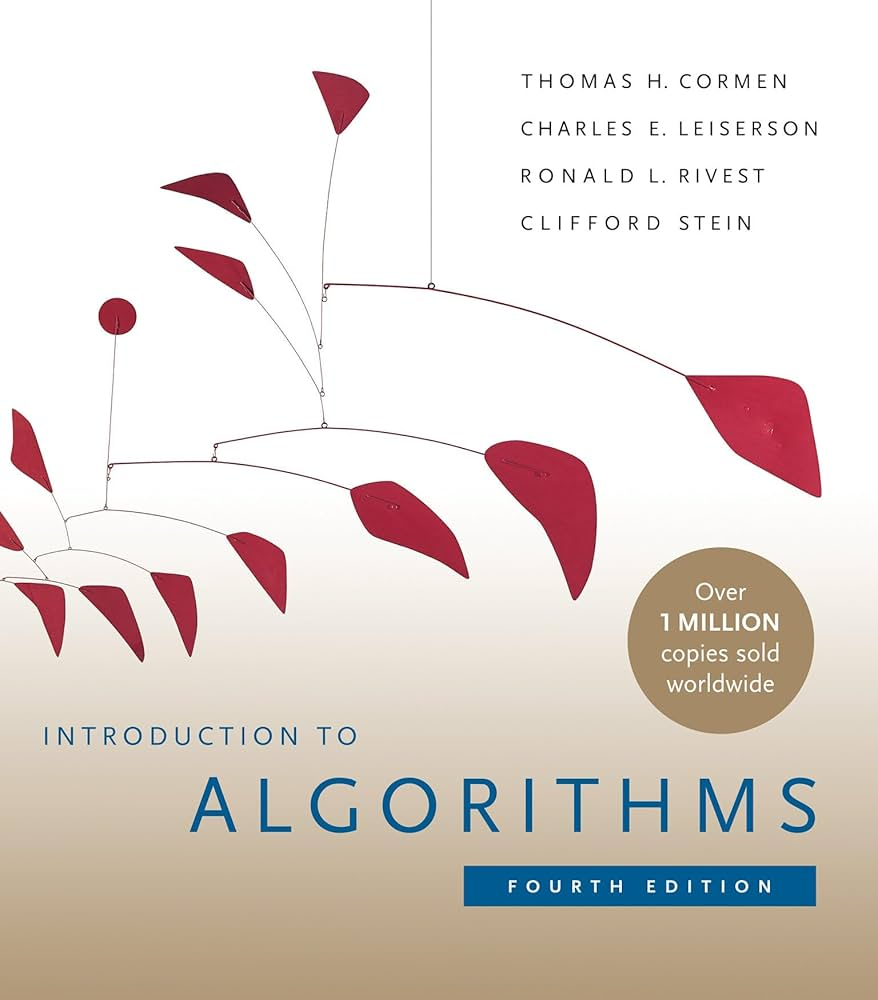
\includegraphics[width=0.45\textwidth]{figures/book_cover.jpg} \\
    \vspace{5mm}{
        \tiny
        Content has been extracted from \textit{Introduction to Algorithms}, Fourth Edition, by Cormen, Leiserson, Rivest, and Stein. MIT Press. 2022.\\
        Visit \url{https://mitpress.mit.edu/9780262046305/introduction-to-algorithms/}.\\
        Original slides from \textit{Introduction to Algorithms 6.046J/18.401J}, Fall 2005 Class by Prof. Charles Leiserson and Prof. Erik Demaine. MIT OpenCourseWare Initiative available at \url{https://ocw.mit.edu/courses/6-046j-introduction-to-algorithms-sma-5503-fall-2005/}.\\
    }
\end{frame}

%\section{Introduction}

\begin{frame}{Introduction}
    Different types of algorithms can be used to solve the all-pairs shortest paths problem:
    \begin{itemize}
        \item Dynamic programming
        \item Matrix multiplication
        \item Floyd-Warshall algorithm
        \item Johnson’s algorithm
        \item Difference constraints
    \end{itemize}
\end{frame}

\begin{frame}{Single-Source Shortest Paths}
    \begin{itemize}
        \item Given directed graph $G = (V, E)$, vertex $s \in V$ and edge weights $w : E \rightarrow \mathbb{R}$
        \item Find $\delta(s, v)$, equal to the shortest-path weight $s \rightarrow v, \forall v \in V$ (or $-\infty$ if negative weight cycle along the way, or $\infty$ if no path)
    \end{itemize} \pause
    \bigskip
    \scriptsize
    \centering
    \begin{tabular}{ c | c | c}
        \textbf{Situtation}         & \textbf{Algorithm}                    & \textbf{Time} \\ \hline
        unweigthed ($w = 1$)        & BFS                                   & $O(V + E)$    \\
        non-negative edge weights   & Dijkstra                              & $O(E + V \lg V)$\\
        general                     & Bellman-Ford                          & $O(VE)$       \\
        acyclic graph (DAG)         & Topological sort + one pass of B-F    & $O(V + E)$    \\
    \end{tabular}\\
    \bigskip
    All of the above results are the best known. We achieve a $O(E + V \lg V )$ bound on Dijkstra’s algorithm using \textbf{Fibonacci heaps}.
\end{frame}

\begin{frame}{All-Pairs Shortest Paths (APSP)}
    \begin{itemize}
        \item Given edge-weighted graph, $G = (V, E, w)$.
        \item Find $\delta(u, v)$ for all $u, v \in V$.
        \item A simple way of solving APSP problems is by running a single-source shortest path algorithm from each of the $V$ vertices in the graph.
    \end{itemize}\pause
    \bigskip
    \tiny
    \centering
    \begin{tabular}{ c | c | c | c}
        \textbf{Situtation}         & \textbf{Algorithm}    & \textbf{Time}         & $E=\Theta(V^2)$ \\ \hline
        unweigthed ($w = 1$)        & $|V| + $ BFS          & $O(V E)$              & $O(V^3)$ \\
        non-negative edge weights   & $|V| + $ Dijkstra     & $O(V E + V^2 \lg V)$  & $O(V^3)$ \\
        general                     & $|V| + $ Bellman-Ford & $O(V^2 E)$            & $O(V^4)$ \\
        general                     & Johnson’s             & $O(V E + V^2 \lg V)$  & $O(V^3)$ \\
    \end{tabular}\\
    \bigskip
    \footnotesize
    These results (apart from the third) are also best known --don’t know how to beat $|V| \times Dijkstra$.
\end{frame}

\begin{frame}{Algorithms to solve APSP\footnote{\scriptsize For all the algorithms described, we assume that $w(u, v) = \infty$ if $(u, v) \in E$}}
    Dynamic Programming (attempt 1):
    \begin{enumerate}
    \scriptsize
        \item \textbf{Sub-problems}: $d_{uv}^{(m)} =$ weight of shortest path $u \rightarrow v$ using $\leq$ edges.
        \item \textbf{Guessing}: What's the last edge (x, v)?
        \item \textbf{Recurrence}:
        \begin{equation*}
            \begin{align*}
                d_{uv}^{(m)} &= min( d_{uv}^{(m - 1)} + w(x, v) & \text{ for } x \in V) \\
                d_{uv}^{(0)} &=
                    \begin{cases}
                        0 & \text{ if } u = v. \\
                        \infty & \text{otherwise}.
                    \end{cases}
            \end{align*}
        \end{equation*}
        \item \textbf{Topological ordering}: for $m = 0, 1, 2, . . . , n - 1$: for $u$ and $v$ in $V$.
        \item \textbf{Original problem}: If graph contains no negative-weight cycles (by Bellman-Ford analysis), then shortest path is simple $\Rightarrow \delta(u, v) = d_{uv}^{(n - 1)} = d_{uv}^{(n)} = \cdots$
    \end{enumerate}
\end{frame}

\begin{frame}{Bottom-up via Relaxation Steps\footnote{{\scriptsize In the above pseudocode, we omit superscripts because more relaxation can never hurt.}}}
    \begin{codebox}
        \li \For $m \gets 1$ \To $n$ \By 1
        \li \hspace{0.5cm} \For u in V
        \li \hspace{1.0cm} \For v in V
        \li \hspace{1.5cm} \For x in V
        \li \hspace{2.0cm} \If $d_{uv} > d_{ux} + d_{xv}$
        \li \hspace{2.5cm} $d_{uv} = d_{ux} + d_{xv}$
    \end{codebox}
\end{frame}

\begin{frame}{Time complexity}
    \begin{itemize}
        \item In this Dynamic Program, we have $O(V^3)$ total sub-problems.
        \item Each sub-problem takes $O(V)$ time to solve, since we need to consider $V$ possible choices.
        \item This gives a total runtime complexity of $O(V^4)$.
        \item Note that this is no better than $|V| \times$ Bellman-Ford.
    \end{itemize}
\end{frame}

\begin{frame}{Matrix Multiplication}
    Recall the task of standard matrix multiplication:
    \begin{itemize}
        \item Given $n \times n$ matrices $A$ and $B$, compute $C = A \cdot B$, such that $c_{ij} = \sum_{k=1}^{n} a_{ik} \cdot b_{kj}$. \pause
        \begin{enumerate}
            \item $O(n^3)$ using standard algorithm. \pause
            \item $O(n^{2.807})$  using Strassen algorithm. \pause
            \item $O(n^{2.376})$  using Coppersmith-Winograd algorithm. \pause
            \item $O(n^{2.3728})$ using Vassilevska-Williams algorithm.
        \end{enumerate}
    \end{itemize}
\end{frame}

\begin{frame}{Connection to Shortest Paths}
    \begin{itemize}
        \item Let's define $\oplus = \min$ and $\odot = +$.
        \item Then, $C = A \odot B$ produces $c_{ij} = \min_k (a_{ik} + b_{kj})$.
        \item Define $D^{(m)} = (d_{ij}^{(m)})$, $W = (w(i, j))$, $V = \{1,2, \ldots, n\}$
    \end{itemize}
    \bigskip
    With the above definitions, we see that $D^{(m)}$ can be expressed as $D^{(m-1)} \odot W$. In other words, $D^{(m)}$ can be expressed as the circle-multiplication of $W$ with itself $m$ times.
\end{frame}

\begin{frame}{Matrix Multiplication Algorithm}
    \begin{itemize}
        \item $n - 2$ multiplications $\Rightarrow O(n^4)$ time (still no better). \pause
        \item Repeated squaring: $((W^2)^2)^{2 \cdots}$ \pause $= W^{2^{\lg n}}$ \pause $= W^{n - 1} = (\delta(i, j))$ if no negative-weight cycles. \pause
        \item Time complexity of this algorithm is now \textcolor{red}{$O(n^3 \lg n)$}.
    \end{itemize}
\end{frame}


\begin{frame}{Floyd-Warshall Algorithms}
    Dynamic Programming (attempt 2):
    \begin{enumerate}
        \item \textbf{Sub-problems}: $c_{uv}^{(k)} =$ weight of shortest path $u \rightarrow v$ whose intermediate vertices $\in \{1,2, \ldots, k\}$ \pause
        \item \textbf{Guessing}:  \pause Does shortest path use vertex $k$? \pause
        \item \textbf{Recurrence}:
        \begin{equation*}
            \begin{align*}
                c_{uv}^{(0)} &= w(u, v) \\
                c_{uv}^{(k)} &= \min(c_{uv}^{(k-1)}, c_{ux}^{(k-1)} + c_{xv}^{(k-1)})
            \end{align*}
        \end{equation*}  \pause
        \item \textbf{Topological order}: for $k$: for $u$ and $v$ in $V$:
        \item \textbf{Original problem}: $\delta(u, v) = c_{uv}^{(n)}$. Negative weight cycle $\Leftrightarrow$ negative $c_{uu}^{(n)}$
    \end{enumerate}
\end{frame}

\begin{frame}{Time Complexity}
    This Dynamic Program contains $O(V^3)$ problems as well. However, in this case, it takes only $O(1)$ time to solve each sub-problem, which means that the total runtime of this algorithm is $O(V^3)$.
\end{frame}

\begin{frame}{Bottom-up via Relaxation}
    \begin{codebox}
        \li $C = (w(u, v))$
        \li \For $k \gets 1$ \To $n$
        \li \hspace{0.5cm} \For u in V
        \li \hspace{1.0cm} \For v in V
        \li \hspace{1.5cm} \If $c_{uv} > c_{uk} + c_{kv}$
        \li \hspace{2.0cm} $c_{uv} = c_{uk} + c_{kv}$
    \end{codebox}
\end{frame}

\begin{frame}{Johnson’s algorithm}
    \begin{enumerate}
        \item Find function $h: V \rightarrow \mathbb{R}$ such that $w_h (u, v) = w(u, v) + h(u) - h(v) \geq 0$ for all $u, v \in V$ or determine that a negative-weight cycle exists.
        \item Run Dijkstra’s algorithm on $(V, E, w_h)$ from every source vertex $s \in V \Rightarrow$ get $\delta_h (u, v)$ for all $u, v \in V$.
        \item Given $\delta_h (u, v)$, it is easy to compute $\delta(u, v)$.
    \end{enumerate}
\end{frame}

\begin{frame}{Proof}
    \textbf{Claim}. $\delta(u, v) = \delta_h (u, v) - h(u) + h(v)$. \\
    \\
    \textit{Proof}. Look at any $u \rightarrow v$ path $p$ in the graph $G$:
    \begin{itemize}
        \footnotesize
        \item Say $p$ is $v_0 \rightarrow v_1 \rightarrow v_2 \rightarrow \cdots \rightarrow v_k$, where $v_0 = u$ and $v_k = v$.
        \begin{equation*}
            \begin{align*}
                w_h (p) &= \sum_{i = 1}^{k} w_h (v_{i - 1}, v_i) \\
                        &= \sum_{i = 1}^{k} [w(v_{i - 1}, v_i) + h(v_{i-1}) - h(v_i)] \\
                        &= \sum_{i = 1}^{k} w(v_{i - 1}, v_i) + h(v_0) - h(v_k) \\
                        &= w(p) + h(u) - h(v)
            \end{align*}
        \end{equation*}
        \item Hence all $u \rightarrow v$ paths change in weight by the same offset $h(u) - h(v)$, which implies that the shortest path is preserved. \qed
    \end{itemize}
\end{frame}

\begin{frame}{How to find $h$?}
    We know that
        $$w_h (u, v) = w(u, v) + h(u) - h(v) \geq 0$$
    This is equivalent to,
        $$h(v) - h(u) \leq w(u, v)$$
    for all $(u, v) \in V$. This is called a \textbf{system of difference constraints}.
    \begin{tcolorbox}[title=Theorem.]
        If $(V, E, w)$ has a negative-weight cycle, then there exists no solution to the above system of difference constraints.
    \end{tcolorbox}
\end{frame}

\begin{frame}{\textit{Proof}}
    \scriptsize
    Say $v_0 \rightarrow v_1 \rightarrow \cdots \rightarrow v_k \rightarrow v_0$ is a negative weight cycle.\\
    Let us assume to the contrary that the system of difference constraints has a solution; let's call it $h$.\\
    This gives us the following system of equations,

    \begin{equation*}
        \begin{align*}
            h(v_1) - h(v_0) & \leq w(v_0, v_1) \\
            h(v_2) - h(v_1) & \leq w(v_1, v_2) \\
            h(v_3) - h(v_2) & \leq w(v_2, v_3) \\
                            & \vdots \\
            h(v_k) - h(v_{k-1}) & \leq w(v_{k-1}, v_k) \\
            h(v_0) - h(v_k) & \leq w(v_k, v_0) \\
        \end{align*}
    \end{equation*}

    Summing all these equations gives us
    $$
        0 \leq w(cycle) < 0
    $$
    which is obviously not possible. \\
    From this, we can conclude that no solution to the above system of difference constraints exists if the graph $(V, E, w)$ has a negative weight cycle. \qed
\end{frame}

\begin{frame}{}
    \begin{tcolorbox}[title=Theorem.]
        If $(V, E, w)$ has no negative-weight cycle, then we can find a solution to the difference constraints.
    \end{tcolorbox}
    \scriptsize
    \textit{Proof}. Add a new vertex $s$ to $G$, and add edges $(s, v)$ of weight $0$ for all $v \in V$.
    \begin{itemize}
        \item Clearly, these new edges do not introduce any new negative weight cycles to the graph.
        \item Adding these new edges ensures that there now exists at least one path from $s$ to $v$. This implies that $\delta(s, v)$ is finite for all $v \in V$
        \item We now claim that $h(v) = \delta(s, v)$. This is obvious from the triangle inequality: $\delta(s, u) + w(u, v) \geq \delta(s, v) \Leftrightarrow \delta(s, v) - \delta(s, u) \leq w(u, v) \Leftrightarrow h(v) - h(u) \leq w(u, v)$. \qed
    \end{itemize}
\end{frame}

\begin{frame}{Time Complexity}
    \begin{enumerate}
        \item The first step involves running Bellman-Ford from $s$, which takes $O(VE)$ time.  We also pay a pre-processing cost to reweight all the edges ($O(E)$). \pause
        \item We then run Dijkstra's algorithm from each of the $V$ vertices in the graph; the total time complexity of this step is $O(VE + V^2 \lg V)$. \pause
        \item We then need to reweight the shortest paths for each pair; this takes $O(V^2)$ time. \pause
    \end{enumerate}
    The total running time of this algorithm is \textcolor{red}{$O(VE + V^2 \lg V)$}.
\end{frame}

























\begin{frame}{}
\end{frame}

% \begin{frame}{}
%    \begin{minted}
%    [tabsize=4, obeytabs, frame=lines, framesep=2mm, baselinestretch=1.2, bgcolor=LightGray, fontsize=\scriptsize]{sql}
%    \end{minted}
% \end{frame}

%     \begin{codebox}
%         \Procname{$\proc{Insertion-Sort}(A)$}
%         \li \For $j \gets 2$ \To $\id{length}[A]$
%         \li \Do
%         $\id{key} \gets A[j]$
%         \li \Comment Insert $A[j]$ into the sorted sequence
%         $A[1 \twodots j-1]$.
%         \li $i \gets j-1$
%         \li \While $i > 0$ and $A[i] > \id{key}$
%         \li \Do
%         $A[i+1] \gets A[i]$
%         \li $i \gets i-1$
%         \End
%         \li $A[i+1] \gets \id{key}$
%         \End
%     \end{codebox}

\begin{frame}{}
    \centering
    \Huge End of Lecture 5.
\end{frame}

\section*{Takeaways}

% Tim Duncan's Top 5 Fundamental Takeaways of the Today's Class
\begin{frame}{TDT5FTOTTC}
    \centering
    
\includegraphics[width=0.75\textwidth]{figures/tim.png}
\end{frame}

\begin{frame}{Top 5 Fundamental Takeaways}
    \small
    \begin{enumerate} \pause
        \item[5]
    \end{enumerate}
\end{frame}

\begin{frame}{Introduction to Algorithms}
    \centering
    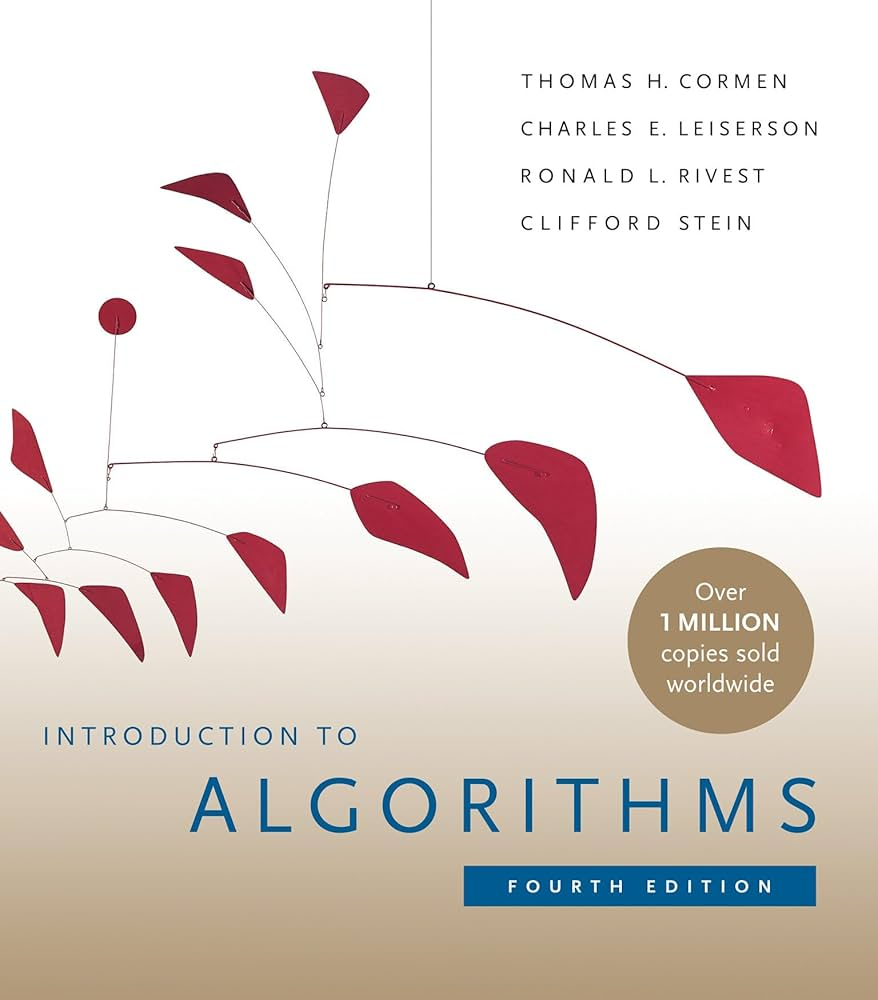
\includegraphics[width=0.45\textwidth]{figures/book_cover.jpg} \\
    \vspace{5mm}{
        \tiny
        Content has been extracted from \textit{Introduction to Algorithms}, Fourth Edition, by Cormen, Leiserson, Rivest, and Stein. MIT Press. 2022.\\
        Visit \url{https://mitpress.mit.edu/9780262046305/introduction-to-algorithms/}.\\
        Original slides from \textit{Introduction to Algorithms 6.046J/18.401J}, Fall 2005 Class by Prof. Charles Leiserson and Prof. Erik Demaine. MIT OpenCourseWare Initiative available at \url{https://ocw.mit.edu/courses/6-046j-introduction-to-algorithms-sma-5503-fall-2005/}.\\
    }
\end{frame}

\end{document}
